\section{Planteamiento del desarrollo del proyecto}
Antes de iniciar con el desarrollo del proyecto, se procedió con una investigación sobre las estructuras de datos que se utilizarían basados en las recomendaciones realizadas previo desarrollo del mismo.

Los cuatro pilares sobre los que se sustenta el presente proyecto son los siguientes:
\begin{itemize}
    \item Lectura y manejo de los archivos a procesar.
    \item Grafos como representación de las relaciones entre archivos.
    \item Índice invertido como estructura de datos para almacenar las palabras relevantes.
    \item PageRank como algoritmo para calcular la importancia de cada archivo dentro del grafo.
\end{itemize}

\subsection{Manejo de archivos}
La idea base consistía en investigar cómo crear una función de manejo de archivos para identificar los archivos regulares de texto plano en el directorio de entrada y sus sub-directorios para posteriormente procesarlos de manera eficiente, evitando la lectura de archivos que no sean de interés.

Se planteó usar una LES (lista enlazada simple) para almacenar los archivos, la cual lleve información de todos los archivos que se encuentran en el directorio de entrada, y a la que se haga referencia (mediante punteros) en las demás estructuras de datos. Esto permite una búsqueda más eficiente y sin un límite de memoria.

\subsection{Grafos}
Como requisito para el funcionamiento del programa es necesario crear un grafo para representar las relaciones entre los archivos y sus contenidos. Se plantearon tres estrategias para crear el grafo, de las que se analizan sus ventajas y desventajas a continuación:
\begin{itemize}
    \item \textbf{Grafos con matriz de adyacencias}: Esta estrategia consiste en crear una matriz de tamaño $n$ (donde $n$ es la cantidad de archivos) para almacenar en ella la información de las relaciones entre los archivos.
    Este tipo de acercamiento favorece la eficiencia en tiempos de lectura y escritura sin embargo presenta dos grandes dificultades:
    \begin{enumerate}
        \item \textbf{Costo de memoria}: El uso de una matriz de tamaño $n$ para almacenar la información de las relaciones entre los archivos implica un costo de memoria considerable guardando espacio en memoria para cada enlace \textbf{aunque no exista}.
        \item \textbf{Memoria adyacente}: Este tipo de sistema requiere un espacio de $n^2\times(\text{tamaño de cada enlace})$ para almacenar la información de las relaciones entre los archivos, lo cual puede suponer una perdida de control para una gran cantidad de elementos.
    \end{enumerate}
    \item \textbf{Grafos con listas de adyacencias}: En esta implementación se plantea el uso de un arreglo o LES de \textit{nodos}, donde cada uno de ellos lleva en sí una LES con sus adyacencias y otra con sus incidencias (nodos que apuntan a esta). Este tipo de estructura de datos permite un manejo de memoria muy preciso, sin embargo en caso de usar arreglos requiere de un espacio de memoria alto, y en caso de usar LES sacrifica la eficiencia en tiempos de lectura y escritura.
    \item \textbf{Grafos con Tablas Hash} Finalmente aparece la opción de usar una Tabla Hash para almacenar la información del grafo. Este tipo de estructura de datos usa una función de \textit{hashing}\footnote{Función que asigna un valor a un objeto de forma que sea única en un conjunto de objetos, es posible que a dos objetos se les asigne el mismo valor a lo que se le conoce como una \textit{Colisión}, este caso debe ser manejado de alguna manera en el uso de tablas hash.} a cada nodo, permitiendo una búsqueda mucho más eficiente (usando como objeto para el hashing el nombre de cada archivo). En los casos que hubieran colisiones dentro de la tabla hash estas se manejan mediante LES que permiten una navegación sencilla entre los nodos con el mismo valor de hash.
\end{itemize}

\subsection{Indice invertido}
El índice invertido es una estructura de datos que almacena los archivos que contienen datos específicos, en lugar de listar los contenidos de cada archivo.

Este enfoque es útil para trabajar con grandes volúmenes de información, ya que facilita la búsqueda y la relación entre los archivos y su contenido.

Para el desarrollo de este proyecto se plantea el uso de un índice invertido para almacenar las palabras relevantes dentro del directorio de entrada. Para cada una de estas palabras se busca almacenar una lista con los archivos que la contienen, facilitando una búsqueda eficiente y basada en palabras claves.

Para implementar esto, surgieron diversas estructuras de datos factibles a utilizar, sin embargo, por las razones mencionadas anteriormente se decidió usar de igual forma una \textit{Tabla Hash} variando las estructuras usadas como se detalla más adelante.

\subsection{PageRank} \label{Subsec:PageRank}
Es estrictamente necesaria para este proyecto la utilización de un algoritmo que permitiera ``rankear'' por importancia cada uno de los nodos del grafo de archivos; lo anterior con el fin de mostrar los archivos relevantes para el usuario a la hora de hacer una búsqueda. Para ello se optó por utilizar el algoritmo de \textit{PageRank}.

PageRank es un algoritmo creado por \textcite{PageRankArticle} que calcula la importancia de un archivo dentro de un conjunto de archivos (planteado inicialmente para el uso sobre páginas web).

``\textit{Se considera que un archivo tiene gran prioridad si es enlazado por archivos de gran prioridad}''. Aunque esta primicia suene redundante, esta es la base del algoritmo, ya que esta ``importancia'' está relacionada con la cantidad de enlaces adyacentes e incidentes que tiene cada archivo.

La fórmula para calcular la importancia esta dada por:
\begin{equation}
PR(i) = \frac{1-d}{n} +d\left( \sum\limits_{i \in B_{i}}^{} \frac{PR(j)}{L(j)} +\frac{S}{N} \right)
\label{eq:PageRank}
\end{equation}
Donde:
\begin{itemize}
    \item $PR(i)$: Page rank de la página $i$.
    \item $d$: Damping Factor o factor de amortiguación.
    \item $N$: Corresponde al numero total de elementos, en este caso archivos.
    \item $B_{i}$ : Cantidad de enlaces adyacentes del archivo $i$.
    \item $PR(j)$: Pagerank de los archivos $j$ que enlazan al archivo $i$
    \item $L(j)$: Número de enlaces adyacentes del archivo $j$.
    \item $S$: Corresponde a la suma de los PageRank de los nodos sin enlaces adyacentes.
\end{itemize}

Esta formula fue extraída del articulo original publicado por los autores de dicho algoritmo \cite{PageRankArticle}, sin embargo, en el presente proyecto fue ligeramente modificada con el fin de mantener consistencia al manejar los archivos que no referencian a ningún otro, es decir \textbf{sin enlaces adyacentes}. Se decidió optar por esta solución debido al poco coste de implementación que representa.

Para explicar la interpretación del algoritmo, se utilizará la analogía presente en el siguiente articulo escrito por \textcite{IntroduccionPageRank}, la cuál imagina a un surfista, el cuál se encuentra navegando entre las diferentes páginas (en este caso archivos) de manera aleatoria. Lo que se busca con esto es construir una matriz con las probabilidades de escoger cada salto entre los archivos, según los enlaces presentes en estos. Dicho articulo profundiza en el trasfondo matemático del algoritmo, sin embargo, como este no es el objetivo del presente informe, únicamente se dejará la interpretación del \textbf{PageRank} de un archivo como la probabilidad que existe de que aquel surfista se encuentre en dicho archivo en un momento dado.

Una representación visual del funcionamiento del algoritmo se puede observar en la figura \ref{fig:page_rank}, la cual muestra un grafo de archivos con sus respectivos enlaces. Esta figura y ejemplo fue recuperada y adaptada del video creado por \textcite{PageRankVideo}.

\begin{figure}[h!]
    \centering
    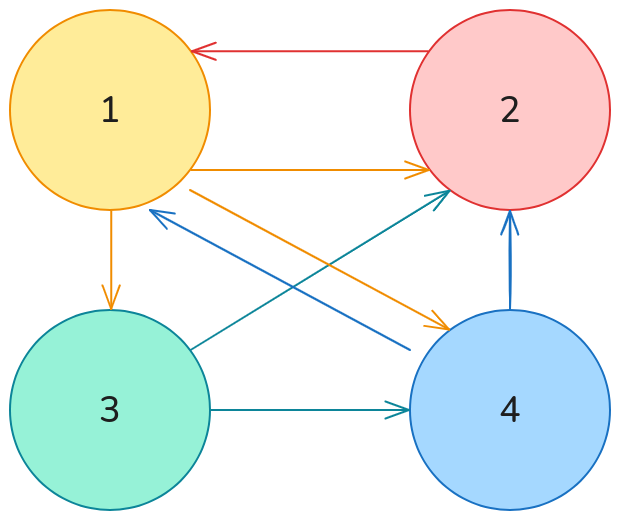
\includegraphics[width=0.4\textwidth]{src/figures/pageRank.png}
    \caption{Representación visual del comportamiento de PageRank}
    \label{fig:page_rank}
\end{figure}

Si se toma cada uno de los nodos con un valor de relevancia inicial $1$, este valor se reparte entre los nodos adyacentes; al resolver el sistema de ecuaciones lineales que resulta de esto, se puede observar que el nodo $1$ cuenta con $\frac{48}{31}$ de relevancia, el nodo $2$ con $\frac{16}{31}$, el nodo $3$ con $\frac{36}{31}$ y el nodo $4$ con $\frac{24}{31}$, como se puede observar, si se suman todas las relevancias, se cuenta con el total de relevancias iniciales que seria $4$, mostrándose asi un breve ejemplo de como se calcula el \textbf{PageRank} de cada nodo.